\chapter{Background}
\label{chap:background}

\section{Distributed Consensus}

Distributed consensus is often based on asynchronous state machine replication.
In this model, each node in the cluster has one instance of a state machine running.
Instructions to this state machines are replicated across the instances, making sure that the order matches for all the state machines.
Since the start state is also specified, this means we will have exactly the same state on each node after a given number of instructions have been executed.

Typical replication protocols provide $2n + 1$ replication, meaning a cluster can stay alive as long as a majority of nodes is alive.
For example, if there is 5 nodes in the cluster, up to two could go offline without impacting the availability or the consistency of the data.
One downside of this is that as the number of node increases, the network load will also increase with it.

\subsection{Raft Consensus Protocol}

Raft\cite{raft} is a protocol that proposes a solution to the distributed consensus problem.
Its main goal is to be easy to understand while still being efficient.
It achieves its objective by cleanly separating different concerns of the protocol.
It also provides a strong leader, i.e. all entries flow from the leader to the followers, making it simpler to reason about.
Unlike the original Paxos, Raft provides a complete solution to build a replicated log.

At its core, Raft is made of three different parts: leader election, log entries replication and commit propagation.
Each node can be in one of three states: \emph{follower}, \emph{candidate} or \emph{leader}.
During normal operation (when a leader emerged), a cluster contains exactly one leader and zero candidates.
We will start by assuming that everything is normal to explain how the protocol works, then explain what changes during leader election.

One important concept in Raft is the \emph{term}.
One term is defined as a period of time in which there is at most one leader.
This means that in order to change the leader, a new term must be changed.
This is implemented through the term number, an always increasing counter.
Note that not all terms have leader, for example if no leader could be elected, the term number is increased before starting a new round of elections.

Each entry in the Raft replicated log is tagged with an \emph{index}, which is a monotonic counter, and the term number.

\subsection{Log Replication}

When the leader receives a request from a client, it appends it to its local log, along with its index and term.
It will then periodically send \emph{AppendEntries} requests to the followers.
Each of those contains all the entries that were not yet acknowledged by the destination follower.
It also contains the term and index of the entries immediately before the first one in the request.
This allows a follower to detect any gap between its local log and the incoming entries.

The destination follower will then append the new entries contained in the \emph{AppendEntries} request to its own log.
During this step, the entries' terms and indices are used to detect inconsistencies and duplicated entries.
It then sends a reply to the leader to acknowledge that the incoming entries were correctly replicated.
It can also notify the leader of a failure to replicate, for example due to a gap in the log.

Note that the checks performed when processing \emph{AppendEntries} requests guarantee that, if two log entries on two different machines have the same index and term, then:

\begin{enumerate}
    \item They store the same operation.
    \item All previous log entries are identical in the two logs.
\end{enumerate}

Those two properties are very useful when considering committing.

\subsection{Entries commit}

We say that an entry is \emph{committed} when we know for sure that this entry will never be lost by the cluster\footnote{Provided that a majority of server stay healthy.}.
We also know that a committed entry will eventually be replicated to the whole cluster.
This means that to be committed, an entry must be replicated on a majority of servers.
When an entry is marked as committed, its content can be consumed by the application.

Raft does not keep track of the commit status for each individual entry.
Instead, it tracks the last committed entry and defines that entries before it are committed as well.

The leader keeps track of the latest acknowledged entry for each follower.
Once an entry has been replicated on a majority of machines, the leader moves its commit index to it, and tells the followers about the new commit index.


\subsection{Leader Election}

In Raft, leader election is based on timers.
First, a periodic timer is used to send heartbeats to followers.
Those heartbeats are \emph{AppendEntries} requests, which can be empty if there is no new request to replicate.
Every time one of those heartbeats is received, the follower resets the second timer, called the \emph{election timeout} timer.

If no messages is received from the leader, then the election timer will fire.
The follower can then then start a new leader election.
It will first increment the term, as there can be only one leader per term.
It will then transition to the candidate state and send \emph{Vote} requests to other cluster participants.

Once a node receives a \emph{Vote} request, it decides wether or not to grant its vote to the requesting candidate.
To do so, it will first check that the candidate's term is more recent than its own.
It will also check that the candidate's log is at least as complete as its own
\footnote{This ensures that the leader's log contains all committed entries.
    If this was not the case, then the leader would start replacing committed entries, leading to loss of consistency.
}.
Finally, it sends a reply to the candidate containing wether or not it grants its vote to the candidate.

If a candidate reaches majority, then it transitions to the leader role and starts sending heartbeats.
If no majority emerges, then the election timeout will fire again, restarting the process at a new term.
To avoid conflicting elections where no majority can occur, the timeout duration is randomized, so that election will eventually succeed.


\section{Transport protocols}

% what is a transport protocol
%   Part of the internet infra
%     provides many functionalities: multiplexing, congestion control, reliable delivery, connection establishement, etc
%     handles delivery of the data to the application

Transport protocols build on the the network (IP) layer and provide services to the applications.
The most important service is multiplexing; several application can use the network, and the transport routes information to them.
This is done using port numbers.
Historically, IP was used with two transport protocols: UDP and TCP.

While UDP only provides connection multiplexing, TCP is much more complicated.
It provides a stream interface, which guarantees that bytes that enter the connection will arrive in the same order at the other end (reliable delivery).
In order to do so, TCP uses has to establish a connection and then acknowledge packets.
It also provides congestion control functionality to avoid link saturation.

All those features made TCP the logical choice when sending data on the Internet, which is pretty unreliable.
However, when running inside a datacenter, packet loss or re-ordering is not as likely.
In addition to this, TCP connection tracking requires requires a lot of messages to send some data, increasing latency (Figure~\ref{fig:tcp_lifecycle}).

% 
% historical: tcp and udp
%     nowadays hard to change this due to things such as nat
% 
% new protocols such as quic and 
% 
% need for a RPC protocol, lots used HTTP
% 
% connection handshake: maybe a tcp connection establishment diagram ?


\begin{figure}[h]
    \centering
    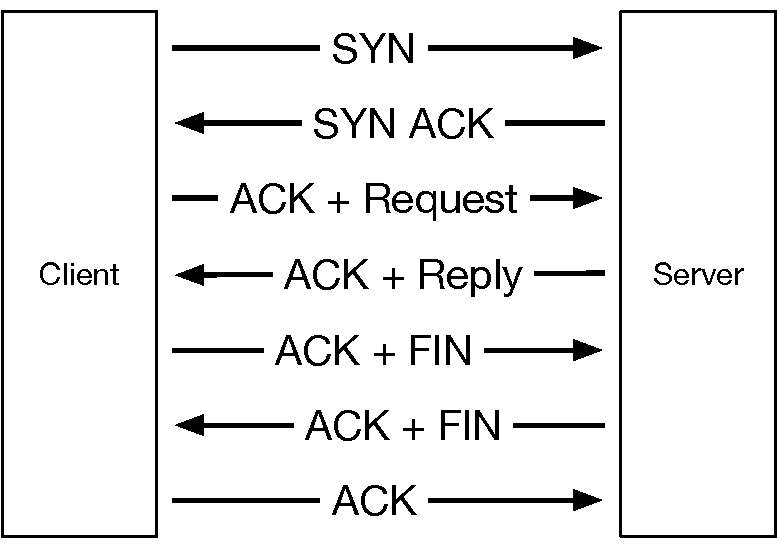
\includegraphics[width=0.4\textwidth]{tcp_lifecycle}
    \caption{Lifecycle of a typical \gls{rpc} over TCP (such as HTTP) interaction.
        We see that the latency before the reply is available takes at least two \gls{rtt}.
    \label{fig:tcp_lifecycle}
    }
\end{figure}


\subsection{Request Response Pair Protocol (R2P2)}

Most current \gls{rpc} systems, such as Google's gRPC\cite{grpc} or Facebook's Thrift\cite{thrift} typically use TCP as their transport layer.
In order to address TCP's shortcomings, the \gls{dcsl} developped a new transport protocol specially designed for \glspl{rpc}.
Unlike TCP, this new protocol is connectionless; each communication is made of a single request followed by a single response, hence the name of \gls{r2p2}.
This reduces latency by removing the handshake round trip time of TCP.

This has been succesfully used in the past to implement new load balancing techniques\cite{r2p2}.
Since it was designed with load balancing, each \gls{r2p2} request includes includes a field to specify how it should be routed.
For example, it can be marked as ``Fixed'', meaning that the request must be served by the receiver, or ``load-balanced'', in which case the router is free to redirect it to another server.
Since \gls{r2p2} has no notion of connections, the reply can be sent directly to the client instead of having an additional trip through the load balancer (Figure~\ref{fig:load_balancing}).

\begin{figure}[h!]
    \centering
    \begin{subfigure}[t]{0.4\textwidth}
        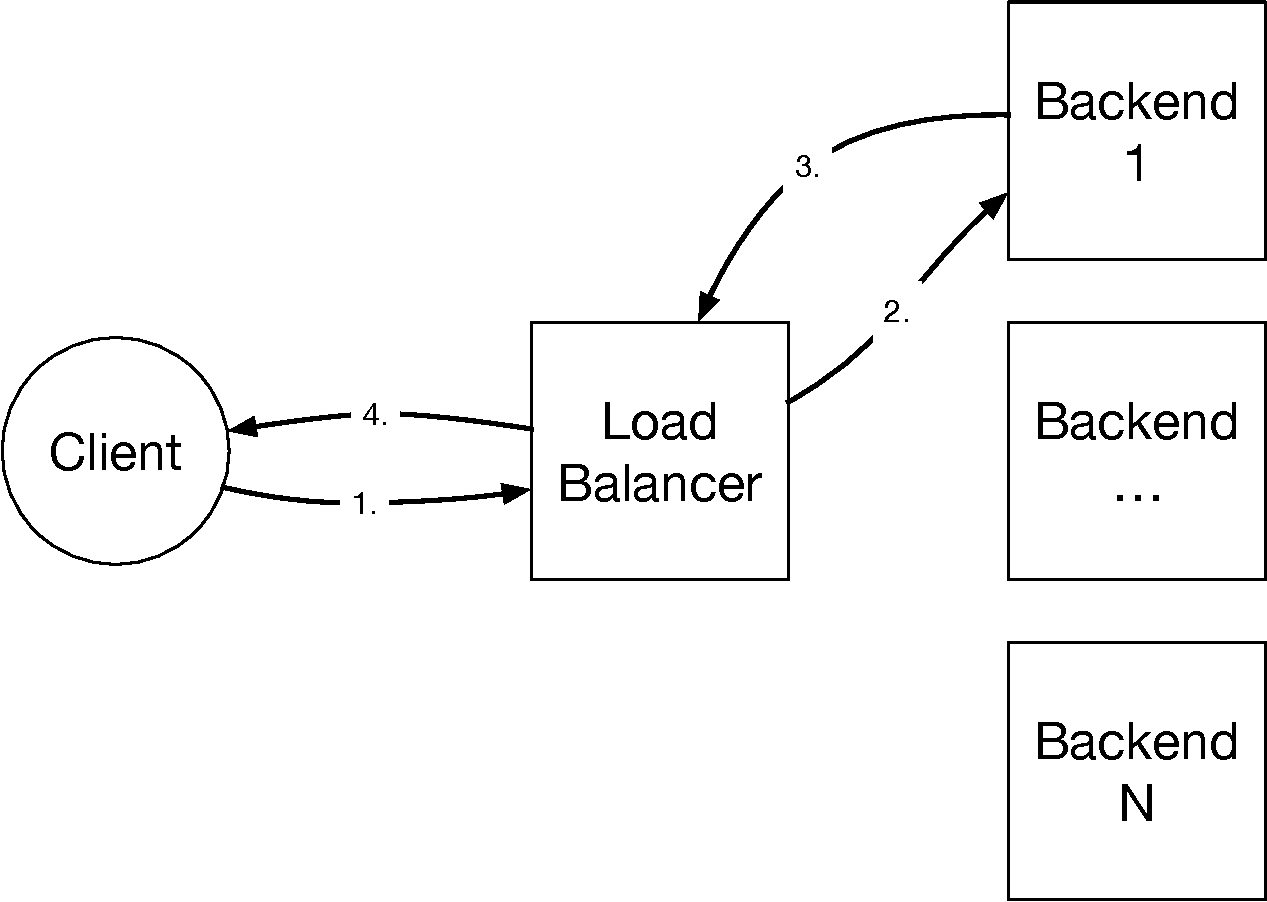
\includegraphics[width=\textwidth]{load_balancer_interaction_tcp.pdf}
        \caption{TCP}
    \end{subfigure}%
    ~
    \begin{subfigure}[t]{0.4\textwidth}
        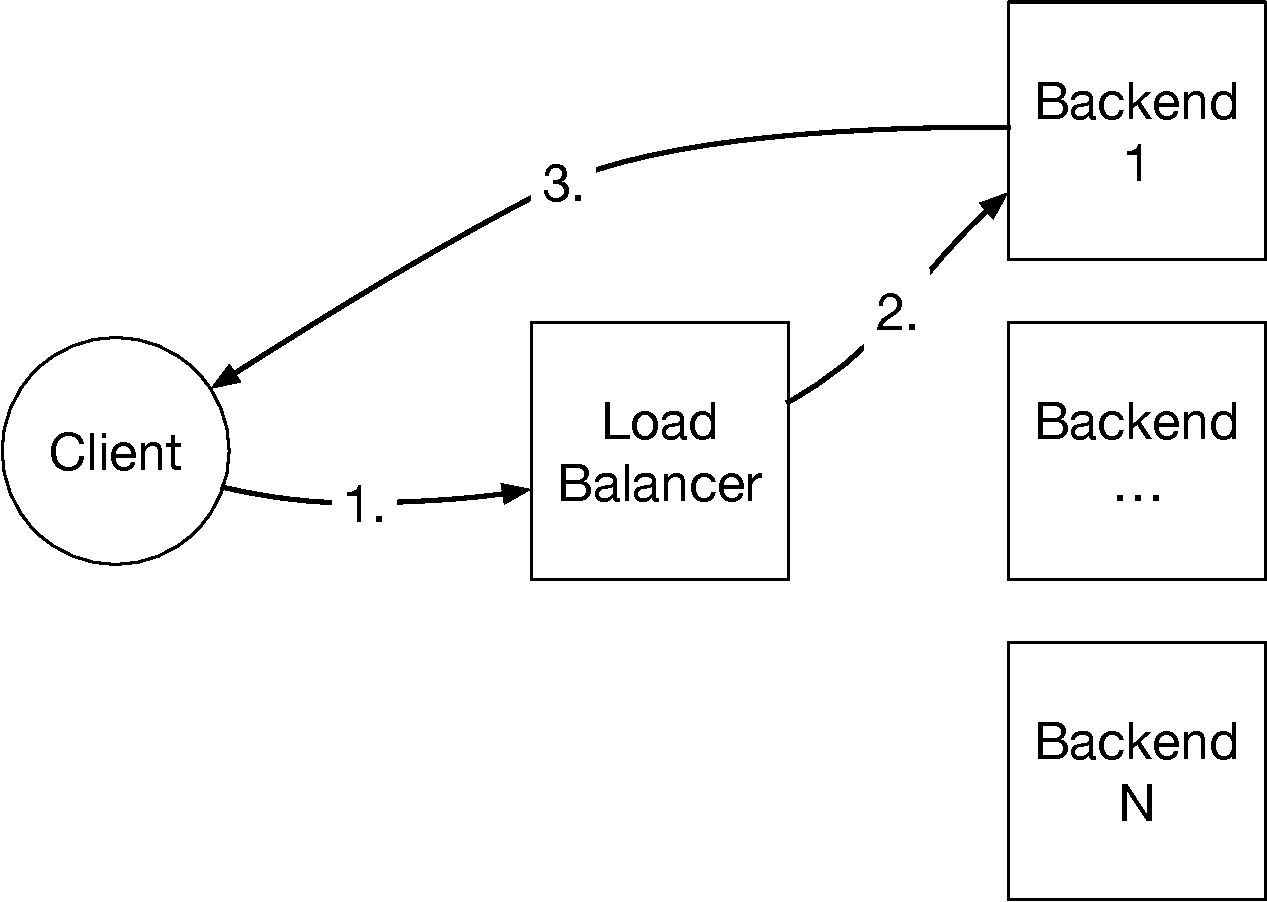
\includegraphics[width=\textwidth]{load_balancer_interaction_r2p2.pdf}
        \caption{\gls{r2p2}}
    \end{subfigure}
    \caption{
        Load balancing data flow using both TCP and \gls{r2p2}.
        We can see that the connection-less nature of \gls{r2p2} allows data to be sent directly back to the client.
        \label{fig:load_balancing}
    }
\end{figure}


We realized that it could be interesting to embed the replication mechanism in the transport layer.
This would greatly simplify the life of the application developer.
Any networked application can be turned into a replicated version of it simply by changing a flag on the requests.
Clients could even choose wether or not to ask for replication based on application-specific logic.
For example, if stales read from a key-value store are acceptable, read request could be marked as ``load-balanced'', while write requests would be marked as ``replicated'' to ensure consistency.


\subsection{R2P2 API}

The \gls{r2p2} library \gls{api} looks nothing like a BSD socket \gls{api}.
Instead it is \emph{event oriented}: the user of the library provides a set of callbacks that are called when a request is received (in the case of a server) or when a response arrives (in the case of a client).
Those callbacks also receive a per-connection argument which can be used to track state.
The core of the \gls{r2p2} \gls{api} can be seen in Listing~\ref{listing:r2p2-client-api} and \ref{listing:r2p2-server-api}.

Such event-oriented \gls{api} maps well to the semantics of either high performance I/O syscalls (e.g. Linux's \texttt{epoll}) or the one of kernel bypass frameworks such as DPDK.

\begin{lstfloat}
\lstinputlisting[label=listing:r2p2-client-api,caption={\gls{r2p2} \gls{api} summary}]{code_snippets/r2p2_client_api.c}
\end{lstfloat}

\begin{lstfloat}
\lstinputlisting[label=listing:r2p2-server-api,caption={\gls{r2p2} server \gls{api}}]{code_snippets/r2p2_server_api.c}
\end{lstfloat}

With our proposal of bringing the consensus protocol to the transport layer, switching a normal application to a distributed, consistent one is simply a matter of changing the \texttt{routing\_policy} field from \texttt{FIXED\_ROUTE} to \texttt{REPLICATED\_ROUTE}.
We hope that this will create a re-usable framework and that more developper will be able to write fault tolerant systems as a result.

\section{Kernel Bypass}

It is well known in the system engineering community that context switching between userland and kernel space can be expensive.
For example, Google observed a 3x gain in throughput when bypassing the Linux kernel\cite{maglev}.

To reduce the number of switches between kernel space and userland, we have two choices: moving more parts of the system in the kernel, or moving more parts of the system in userland.  The first option is the one that has been traditionnaly been used for networking; the TCP/IP stack or the filesystem are part of typical UNIX kernels.
However, moving code in kernel space is not an easy task: kernel code usually has very little to no memory protection.
This causes security threats and makes debugging harder.

The second option, moving more parts of the system in userland is known as \emph{kernel bypass}.
In this technique, the application embeds everything it needs, from \gls{nic} drivers to TCP.
The main downside of this technique is that it prevents sharing of ressources between applications running on the server.
For example, each networked application would need its own \gls{nic}.

A key contribution of our work is the use of kernel bypass techniques to reduce latency.
In particular, we are opposing our design to Kernel Paxos\cite{kernelpaxos}, which moved the Paxos consensus protocol in the Linux kernel with great results.
We believe that using kernel bypass techniques can lead to similar, if not better performance without compromising process separation.


